\chapter{Background}

\section{Formula SAE}
Formula SAE is an international design competition founded by the american Society of Automotive Engineers (SAE) in 1980, in which university students develop, build and race an open-wheel, single seater race car. The car must adhere to the Formula SAE rules that govern all the aspects of the car and the competition.

In Europe, Formula Student Germany (FSG) is the main governing body. FSG releases the rulebook \cite{fsg2020} that is used in all european competitions and it organizes the biggest competition of the season. Many more Formula SAE events are held all around Europe and the world.

\subsection{Competitions}
A Formula SAE competition consists of static and dynamic events in which industry experts judge the cars and the teams on several different aspects by awarding points for each event.

\subsubsection{Tech Inspections}
At the start of the competition technical inspections are carried out to verify that each car is respecting the rulebook and is thus eligible to participate in the dynamic events.
The inspection is carried out as follows:
\begin{itemize}
    \item \textbf{Pre-inspection}: safety hardware, driver equipment, tires and rims are checked for compliance with the SAE and FIA rules.
    \item \textbf{Accumulator inspection}: the battery pack's adherence to the SAE rules is verified by checking its insulation and data acquisition methods. The pack is then sealed for the rest of the competition.
    \item \textbf{Electrical inspection}: all electrical components on the car are checked for compliance ny verifying every component's datasheet. Furthermore, electrical grounding is checked all across the car.
    \item \textbf{Mechanical inspection}: It is verified that the car's dimensions are within rulebook specification. All strength samples for the chassis materials are shown to the officials.
    \item \textbf{Tilt test}: the car with driver is put on an inclined platform with a lateral angle of 60 degrees. The car must adhere to the platform's surface and no fluids must leak.
    \item \textbf{Rain test}: the car is sprinkled with water for 120 s to check proper humidity insulation of electronic components. The car must be on during the test and must remain powered for an additional 120 s.
    \item \textbf{Brake test}: the driver accelerates the car, switch it off and perform an emergency brake test. All four wheels must lock and the car must not deviate its path.
\end{itemize}
If the car passes every step of the tech inspections, it gets certified and can participate in the dynamic events.

\subsubsection{Static Events}
In static events the car and the team are evaluated on theoretical points including design processes, team organization, business ideas and more.
Static events are divided in three separate categories:
\begin{itemize}
    \item \textbf{Engineering design} (150 pts.): The judges evaluate the whole design process of the car, from the early stages of evaluation to the realization and validation of components. Each team's department has to justify all choices made in the design phase with data collected from simulations, previous experience or QFD methodology.
    \item \textbf{Cost and manufacturing} (100 pts.): The team provides an engineering and a manufacturing BOM in which the cost of each component is reported. Team members have to explain the cost of every component, material and manufacturing process.
    \item \textbf{Business plan presentation} (100 pts.): In the business plan presentation judges pretend to be potential investors and the team has to make an enticing presentation of its product and the business model in which the team plans to mass-produce the prototype car with studies on costs and profitability. Innovative and original ideas are usually rewarded.
\end{itemize}

\subsubsection{Dynamic Events}
Dynamic events value the overall performance of the car compared to its competitors. The car is put through four different tests that each assesses a different aspect of performance:
\begin{itemize}
    \item \textbf{Skidpad} (75 pts.): the car must complete two laps of a figure 8 track, sometimes on wet tarmac.
    \item \textbf{Acceleration} (75 pts.): the car must do a standing start and complete a straight 75 m long track as fast as possible.
    \item \textbf{Autocross} (100 pts.): a single lap of an autocross track with a length lower than 1,5 km must be completed in the least time possible. The track contains slaloms, straights and sharp turns.
    \item \textbf{Endurance and efficiency} (425 pts.): the car must race for a total length of 22 km around a track similar to the autocross layout.
\end{itemize}
For each of the previous events, points are calculated based on the time taken to complete the race. For the Endurance event efficiency is also taken into account.

\section{E-Agle Trento Racing Team}
E-Agle Trento Racing Team is the Formula SAE team of the University of Trento. The team was created in 2016, and was immediately involved in the creation of electric race cars. Since its inception, the team realized two Formula SAE cars: Chimera and Chimera Evoluzione. Instead of following an evolutionary approach with the third car, the team decided to design the vehicle from scratch. This choice came from the experience with the two previous cars: some inconvenient design flaws and the will to innovate were the main driving forces of this decision.

The redesign was completed in 2019 with production planned to end in time for the 2020 racing season; unfortunately, due to the COVID-19 pandemic, all competitions were canceled and the team was forced to work away from the workshop. In 2021 production was resumed and the car is planned to compete in the second half of the 2021 season and continue for 2022.

The team is divided in four main divisions, each in charge of a different assembly of the car:
\begin{itemize}
    \item \textbf{Mechanical Team}: is in charge of the design, manufacturing and testing of every mechanical component of the car including the chassis, suspension components, aerodynamics and more.
    \item \textbf{Dynamics and Modeling Team}: the team develops the suspension kinematics and the whole car dynamics based on simulations of a virtual model of the car. By using the same model the team then creates the control logic of the vehicle that includes the traction control and torque vectoring algorithms.
    \item \textbf{Electronics Team}: Fenice relies on custom-designed electronics for most of its features. The team's job is to design and test all the electronic components, from the car's wiring to the high-voltage battery pack, from the printed circuit boards to the complex battery management system inside the high-voltage battery.
    \item \textbf{Software Team}: The award winning cockpit HMI embedded in the steering wheel is fully custom built by the software team along as the telemetry system that provides data logging and live telemetry. In addition the team is responsible for developing the control boards designed by the electronics division.
\end{itemize}

\begin{figure*}[h]
    \centering
    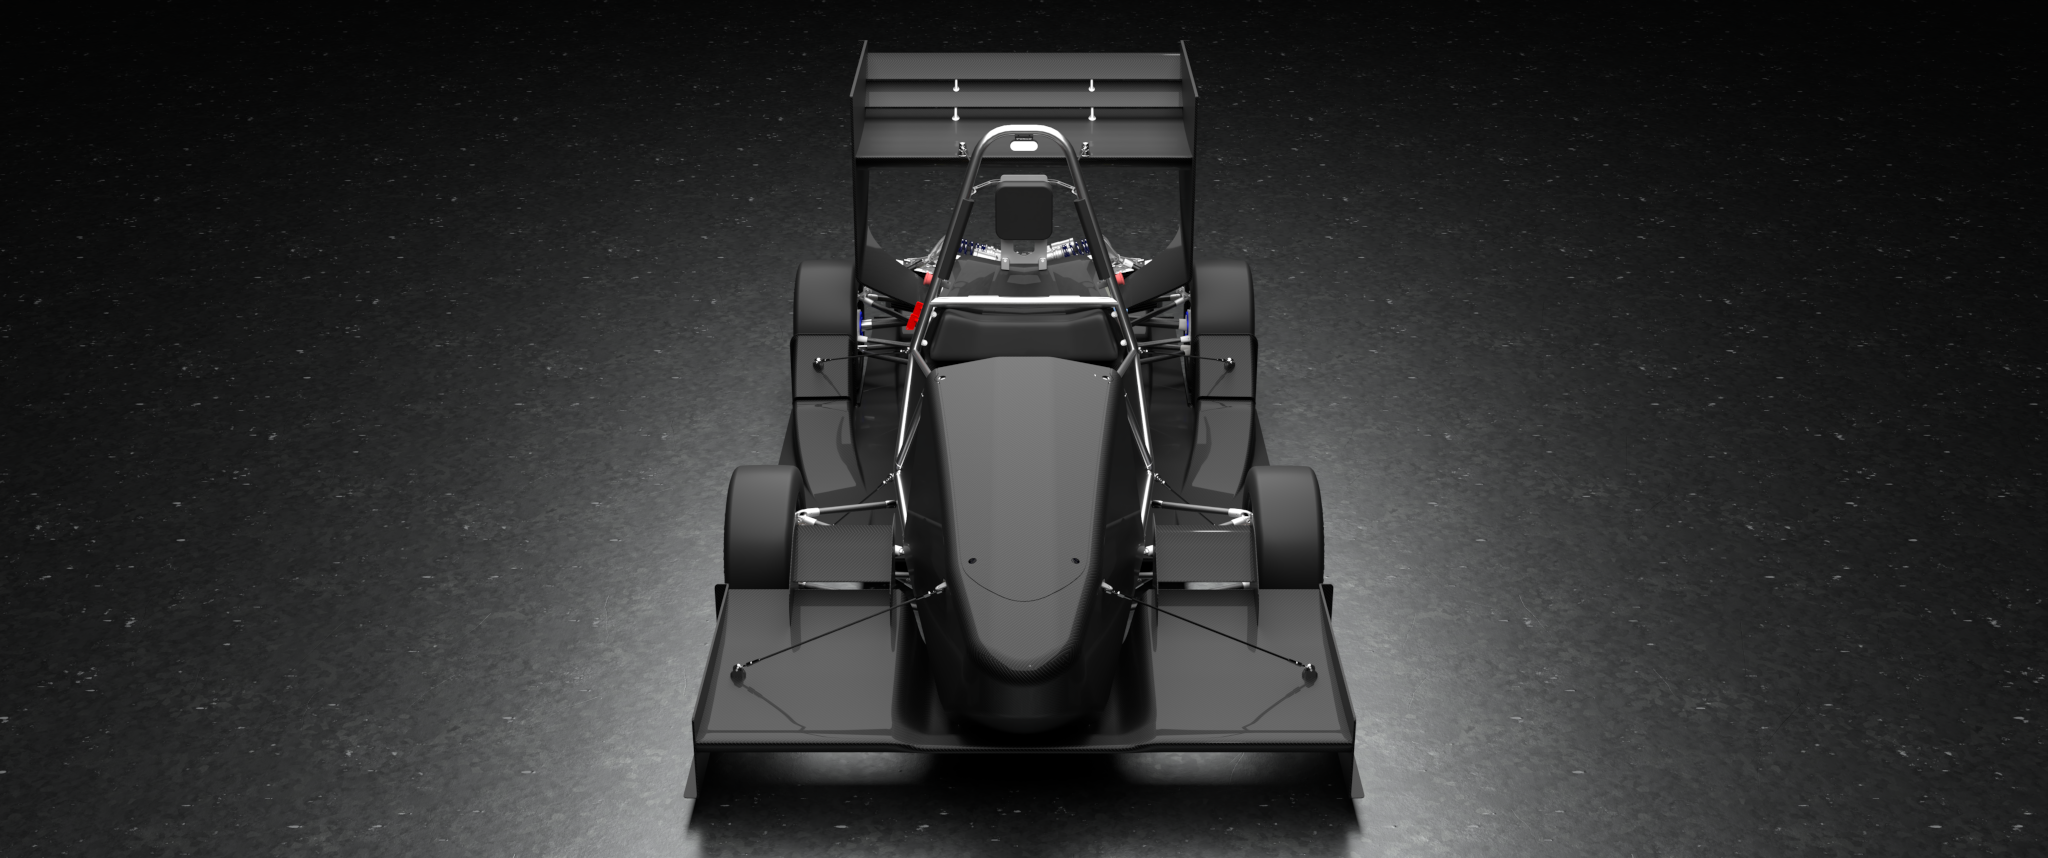
\includegraphics[scale=0.22]{fenice}
    \caption{A render of Fenice}
    \label{fig:fenice_render}
\end{figure*}

\newpage

